%++++++++++++++++++++++++++++++++++++++++
% Don't modify this section unless you know what you're doing!
\documentclass[letterpaper,12pt]{article}
\usepackage[utf8]{inputenc}
\usepackage{float}
\usepackage{tabularx} % extra features for tabular environment
\usepackage{amsmath}  % improve math presentation
\usepackage{graphicx} % takes care of graphic including machinery
\usepackage[margin=1in,letterpaper]{geometry} % decreases margins
\usepackage{cite} % takes care of citations
\usepackage[final]{hyperref} % adds hyper links inside the generated pdf file
\usepackage[table,xcdraw]{xcolor}

\hypersetup{
	colorlinks=true,       % false: boxed links; true: colored links
	linkcolor=blue,        % color of internal links
	citecolor=blue,        % color of links to bibliography
	filecolor=magenta,     % color of file links
	urlcolor=blue        
}

\begin{document}

\title{Práctica 4 - Ruteo Externo}
\author{Matthew Aguerreberry, Natasha Tomattis}
\date{\today}
\maketitle

\section{Practica de Ruteo Externo - BGP}
	\begin{figure}[ht]
			
		\centering 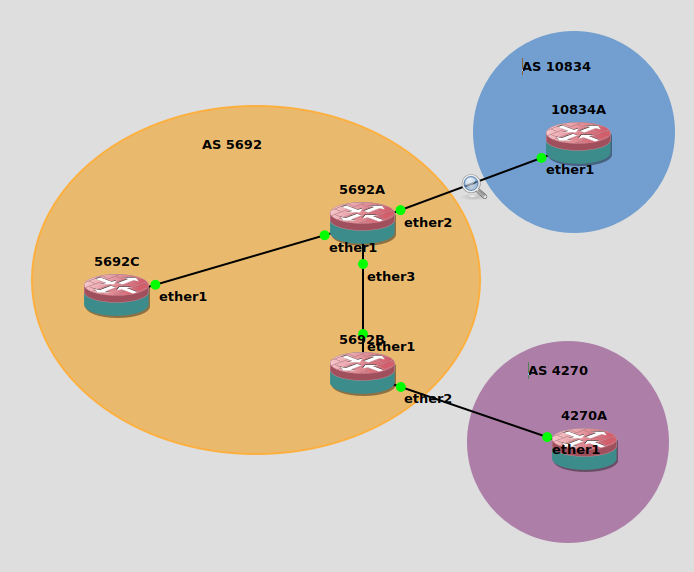
\includegraphics[width=0.6\columnwidth]{figure/bgp-topo.png}
		\caption{
				\label{fig:samplesetup} % spaces are big no-no
				Implementación Topologia 1.
		}
	\end{figure}
	\begin{enumerate}
		\item \textbf{Conectar los routers según el diagrama de la figura 1.}
		\item \textbf{Configurar las interfaces de acuerdo al diagrama. Definir las redes loopbacks para simular redes internas (en el AS 5692 las loopbacks están en el router 5692C).}
		\item \textbf{Configurar eBGP e iBGP según corresponda. Comprobar que se establecen las sesiones correctamente entre los routers vecinos. No habilitar BGP en el router 5692C}
		
		\item \textbf{Que protocolo de capa de transporte utiliza BGP? Que puerto usa? Capturar tráfico para responder estas preguntas}
		Como se aprecia en la captura a continuación, BGP utiliza el puerto bien conocido 179 y trabaja sobre el protocolo de transporte TCP.

		\begin{figure}[H]
			\centering 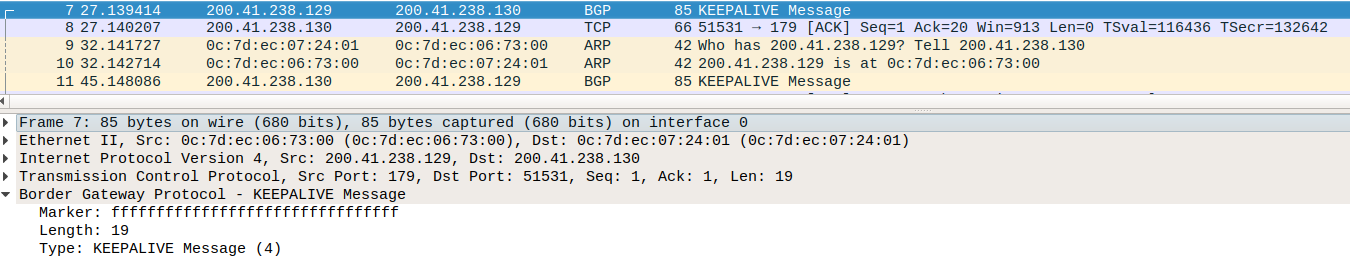
\includegraphics[width=1\columnwidth]{figure/bgp-transport.png}
			\caption{
				\label{fig:samplesetup} % spaces are big no-no
				Captura de mensajes BGP en la interfaz ether2 en el router 5962A.
			}
		\end{figure}
		
		\item \textbf{Que mensajes intercambian dos routers vecinos para establecer una sesión BGP?}\\
		Los vecinos intercambian mensajes de OPEN con el número de AS, el router identifier (la interfaz más baja de la configuradas), la versión de BGP y campos opcionales.

		\begin{figure}[H]
			\centering 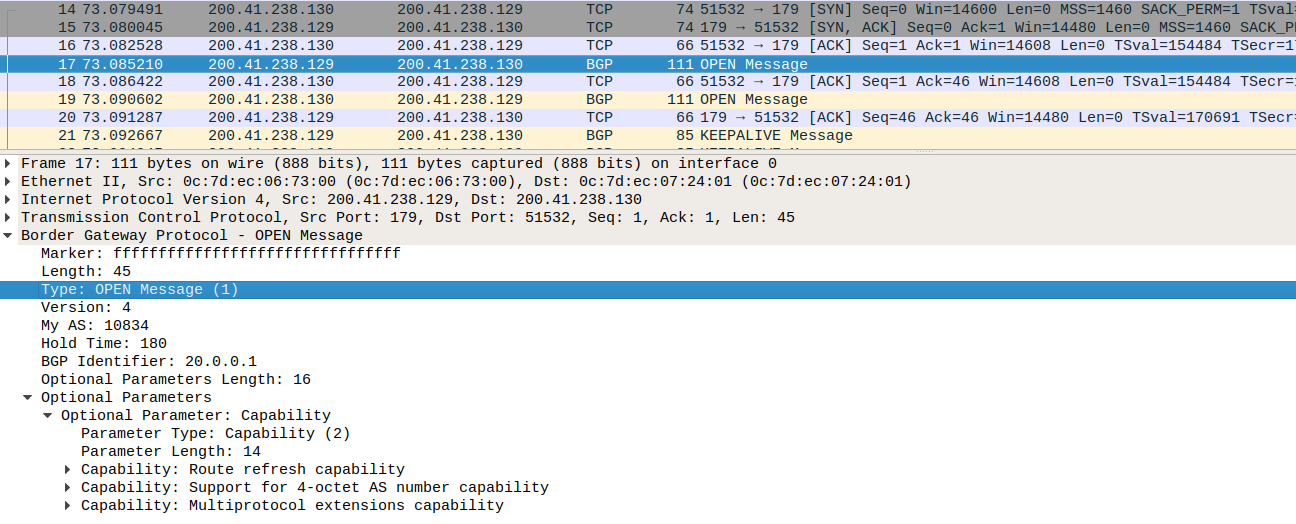
\includegraphics[width=1\columnwidth]{figure/bgp-open.png}
			\caption{
				\label{fig:samplesetup} % spaces are big no-no
				Captura de mensajes BGP en la interfaz ether2 en el router 5962A.
			}
		\end{figure}

		\item \textbf{Cuáles son los estados en los que se puede encontrar una sesión BGP?}\\
		Para operar con sus pares cada router BGP usa una máquina de estado de 6 estados: Idle; Connect; Active; OpenSent; OpenConfirm; y Established.
	
		\item \textbf{¿Qué datos lleva un mensaje UPDATE para informar una ruta? ¿Y para removerla? Capturar trafico entre los routers 5692A y 10834A, remover y volver a agregar la ruta 20.0.0.0/8.}\\
		La siguiente imagen muestra los campos de un mensaje UPDATE para informar una nueva ruta. Aquí encontramos la información de como se aprendió la ruta (path attribute - ORIGIN) que en este caso es IGP. Luego, el mensaje nos indica los AS que debemos atravesar para llegar a esta nueva ruta (path attribute - AS\_PATH), en esta caso solo el AS 10834 se encuentra en el camino. Además, encontramos el próximo salto para llegar a la ruta (path attribute - NEXT\_HOP), en esta caso 200.41.238.129. Finalmente, en el campo \textit{Network Layer Reachability Information (NLRI)} se indica la nueva ruta, 20.0.0.0/8 para este caso.

		\begin{figure}[H]
			\centering 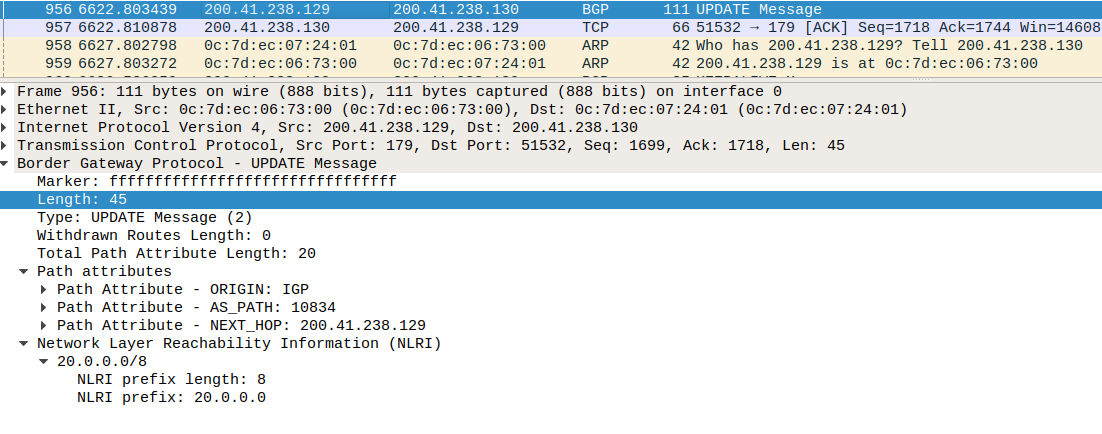
\includegraphics[width=1\columnwidth]{figure/bgp-update.png}
			\caption{
				\label{fig:samplesetup} % spaces are big no-no
				BGP mensaje de UPDATE.
			}
		\end{figure}
		
		\item \textbf{¿Qué significa que el orígen de la ruta sea IGP? ¿Qué otros orígenes pueden existir?}\\
		Que el orígen de la ruta sea IGP quiere decir que la ruta se aprendió internamente en el AS. Los posibles valors del campo ORIGIN son: 0 origen IGP; 1 origen EGP (generalmente BGP); y 2 origen desconocido. 
		
		\item \textbf{¿Cuál es la función de los mensajes KeepAlive?}\\
		Para mantener establecida una sesión BGP. En caso de no recibir ninguno de estos mensajes y expirar el tiempo de \textit{HOLD\_DOWN}, el vecino se declara caído y todas sus rutas son eliminadas.
		
		\item \textbf{Configurar BGP para que se intercambien los prefijos descriptos en el diagrama entre los AS:}
		\begin{enumerate}
			\item \textbf{Resolver en el AS con varios routers el ruteo interno mediante un protocolo IGP (OSPF o RIP).}
			\item \textbf{Ver la tabla de rutas BGP aprendidas y publicadas por cada router.}
			\item \textbf{¿Qué tipos de rutas hay insertadas en la tabla de ruteo? ¿Qué distancia poseen?}\\
			Las rutas aprendidas son de tipo BGP internas y poseen una distancia administrativa de 200.
			
			\begin{figure}[H]
				\centering 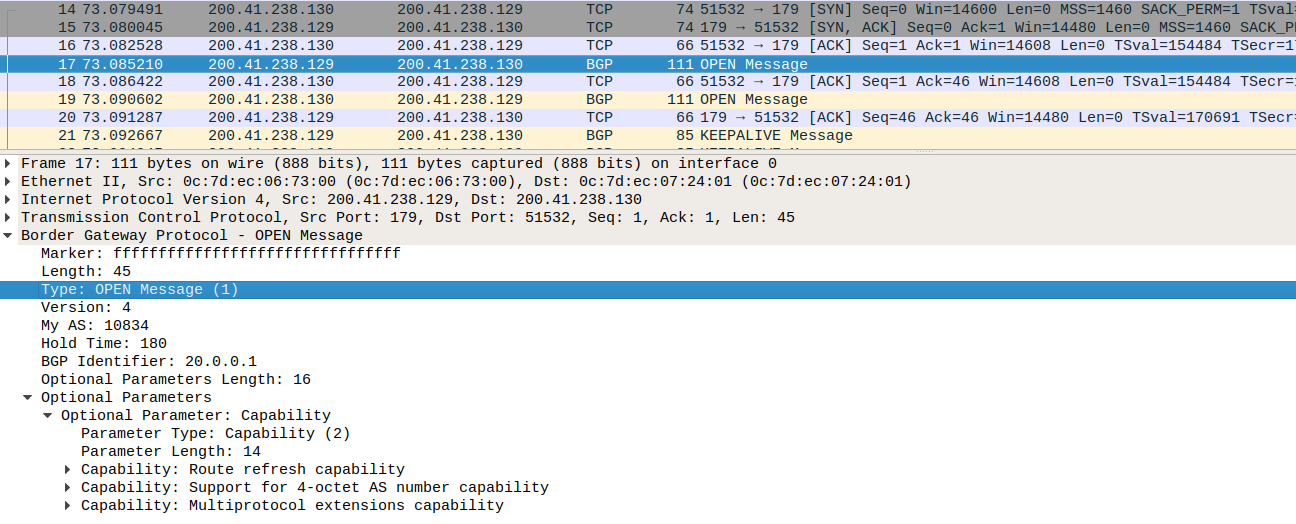
\includegraphics[width=1\columnwidth]{figure/bgp-open.png}
				\caption{
					\label{fig:samplesetup} % spaces are big no-no
					Tabla de rutas BGP del router 5692A.
				}
			\end{figure}
			
			\item \textbf{Probar la conectividad de loopback a loopback con ping (usar el ping extendido para modificar la IP origen de los ICMP)}
			\item \textbf{Si no es posible llegar inspeccionar las tabla de enrutamiento. ¿Qué debería agregar en router 5692C para que llegue a la loopback del AS 10384?}\\
			Al router 5692C se le debe agregar una default gateway a 163.10.199.146, donde se encuentra un router BGP que conoce como enrutar hacia el AS 10834.
			\item \textbf{¿Y para alcanzar la red 70.0.0.0/8 del AS 4270? ¿Por que no aprende el router 5692A la ruta a esa red?}\\
			Para alcanzar la red 70.0.0.0/8 del AS 4270 se debe publicar dicha red por BGP para que el router 5692A la aprenda y sepa routear tráfico hacia ella.
			\item \textbf{¿Qué debería suceder para que las loopbacks de los ASs 10834 y 4270 puedan conectase entre sı? ¿Como debería funcionar el AS 5692?}\\
			El AS 5692 debería ser configurado como AS de tránsito.
		\end{enumerate}
		
		\item \textbf{Configurar el AS 5692 como un AS de transito y probar la conectividad entre los AS externos (usar el atributo next-hop):}
		\begin{enumerate}
			\item \textbf{¿Qué otras opciones podría elegir para hacer lo mismo pero sin utilizar el atributo next-hop?}
			\item \textbf{Publicar desde el AS 10834 un prefijo privado, e.g. 192.168.1.0/24.}
			\item \textbf{Filtrar los prefijos privados de entrada desde el AS 5692.}
			\item \textbf{Publicar un prefijo /27 desde el AS 10834, e.g. 170.210.2.0/27.}
			\item \textbf{Filtrar los prefijos mas largos que 24 de entrada desde el AS 5692.}
			\item \textbf{Anunciar por el IGP dentro del AS 5692 la red 10.0.0.0/24 y filtrarla en la salida BGP.}
			\item \textbf{Pasar el AS 5692 de Transito a Multi-home, Non-Transit.}
		\end{enumerate}
		
		\item \textbf{Priorizar enlaces:}
		\begin{enumerate}
			\item \textbf{Conectar los AS externos al 5692 entre si mediante un nuevo enlace usando la red 80.0.0.0/24}
			\item \textbf{Publicar la red de interconexión por BGP desde los dos enlaces.}
			\item \textbf{Forzar por BGP que el AS 5692 para alcanzar esta red salga por uno de los enlaces.}
			\item \textbf{Forzar por BGP que los AS externos entren al AS 5692 por uno de los enlaces.}
		\end{enumerate}
	\end{enumerate}

	\subsection{Enlaces consultados}
		\begin{itemize}
			\item{HCNA Networking Study Guide}  \\
			\textit{Springer. Huawei Technologies Co., Ltd.},Ch 8.2 RIP.
			\item \href{https://www.juniper.net/documentation/en_US/junos/topics/concept/ospf-stub-áreas-overview.html}
			{Understanding OSPF Stub Areas, Totally Stubby Areas, and Not-So-Stubby Areas}
			\item \href{https://www.juniper.net/documentation/en_US/junos/topics/concept/ospf-routing-external-metrics-overview.html}
			{Understanding OSPF External Metrics}
			\item \href{https://wiki.mikrotik.com/wiki/Manual:Routing/OSPF}
			{Manual:Routing/OSPF}

		\end{itemize}
\end{document}